\documentclass{standalone}
\usepackage{diplomski}

\begin{document}

\chapter{Sensing method}
\pagenumbering{arabic}
\setcounter{page}\thestranica

% --------------------------------------

Optical fibres can be used to measure a variety of physical quantities, utilizing otherwise (i.e. in communication systems) unwanted optical effects that may occur within \cite{krohnFundamentals}. Depending on the sensing method, the obtained results can either be spatially-discrete, if the measurement was localized to a specific point in space, or distributed, if the measurement method yields a profile showing the value of the observed physical quantity at every point of one-dimensional span of the measurement fibre. Some sources categorize optical sensors depending on the modulation localization, thus distinguishing intrinsic sensors -- if the modulation occurs within the fibre -- and extrinsic sensors, with an external transducer of the physical quantity \cite{mitschke2010fiber}. Furthermore, sensors can be categorized depending on the observed optical phenomenon:
\begin{description}
	\item[Phase-modulated] -- The detected signal is usually compared with a reference by interferometric methods.
	\item[Intensity-modulated] -- A form of amplitude modulation by an optical effect.
	\item[Wavelength-modulated] -- Perturbation in the parameter of interest changes physical characteristics of the fibre, inducing a non-linear effect.
	\item[Scattering-based] -- An Optical time-domain interferometer (abbr. OTDR) monitors a backscattered signal produced as a result of intrinsic optical effects.
	\item[Polarization-based] -- Perturbation in the parameter of interest changes the polarization of an incident signal, and causes formation of cross-polarized elements.
\end{description}
Another feature of some fibre-optical sensors is the requirement of reaching the sensing element only from the one side, as opposed to connecting the sensing element at both ends. This is primarily a feature of scattering-based sensors, as only back-scattered signal may be sufficient in determining the required information. Generally, a distributed sensor can function in quasi-distributed, or distributed configuration \cite{Rogers1999}. In a quasi-distributed configuration, couplers are placed at discrete points along the measurement fibre, and terminated in the coupled branch with a totally-reflective device, as presented in Figure \ref{fig:quasi_distributed}.
\begin{figure}[h]
	\centering
	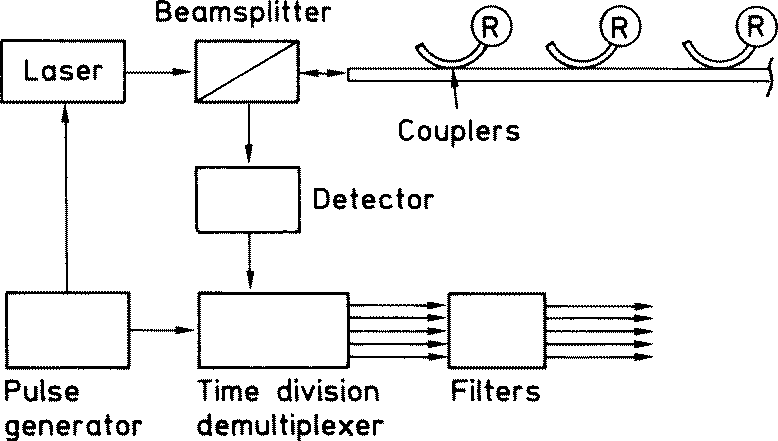
\includegraphics[width=0.6\textwidth]{quasi_distributed.png}
	\caption{Quasi-distributed sensor \cite{Rogers1999}}
	\label{fig:quasi_distributed}
\end{figure}
The measured reflectance can then be time-demultiplexed in order to obtain measurements at multiple discrete points along the fibre. On the other hand, a fully-distributed configuration uses scattering effects within the fibre, and measures the backscattered signal, providing a continuous profile of the measured quantity. The achieved measurement method is OTDR.\\

\section{Optical time-domain reflectometry}

In its elementary form, OTDR is used for characterizing an optical fibre or an optical link along its length \cite{UnderstandingOTDRs2000}. The effect enabling this kind of measurement is the backscattered Rayleigh signal. A block diagram of an OTDR system is shown in Figure \ref{fig:otdr_block}.
\begin{figure}[h]
	\centering
	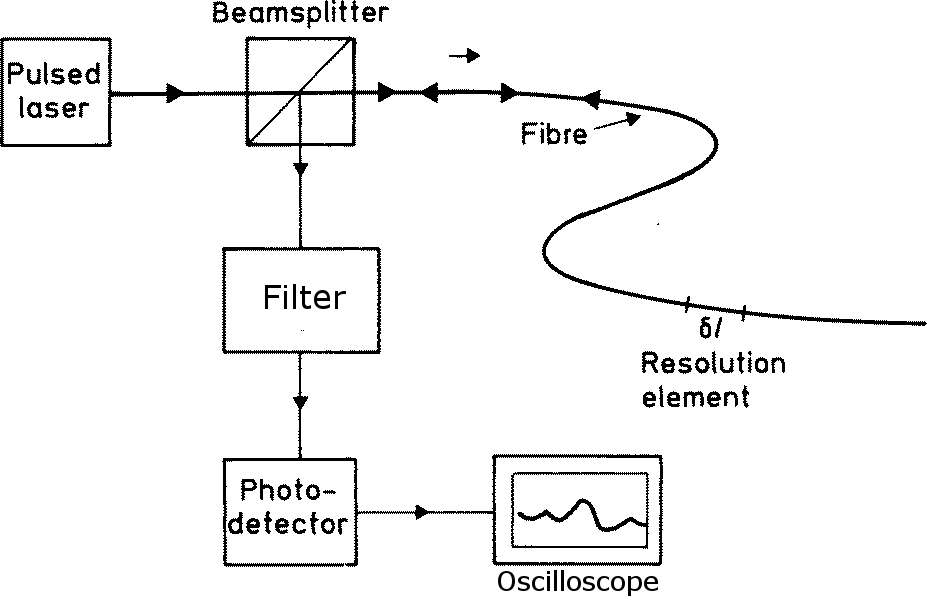
\includegraphics[width=0.7\textwidth]{otdr_block.png}
	\caption{Block diagram of an OTDR system \cite{Rogers1999}}
	\label{fig:otdr_block}
\end{figure}
A laser is placed at the beginning of the measurement fibre, and its optical output coupled to it through a circulator. The measurement fibre is then excited by a laser pulse with an optical signal of power $P_0$, and pulse width $T_0$. As the pulse propagates along the fibre, it will suffer losses determined by the attenuation coefficient $\alpha$. As discussed in chapter \ref{ch:fibres}, a fundamental loss mechanism is Rayleigh scattering. Therefore, it is convenient to represent $\alpha$ as a sum \cite{agrawal}
\begin{equation}
\alpha = \alpha_R + \alpha_a \textrm{,}
\end{equation}
where $\alpha_R$ is the contribution of Rayleigh scattering to total losses. Rayleigh scattering occurs as a result of microscopic fluctuations in density, leading to small perturbations in refractive index. The scattering cross-section is largely dependent on wavelength, so $\alpha_R$ can be expressed as
\begin{equation}
\alpha_R = \frac{C}{\lambda^4} \textrm{.}
\end{equation}
Here, $C$ is a fibre-dependent constant, ranging around $\SI{0.7}{(\decibel / \kilo \meter) \, \micro \meter ^4} < C < \SI{0.9}{(\decibel / \kilo \meter) \, \micro \meter ^4}$, producing a Rayleigh-limited attenuation coefficient around $\SI{0.12}{\decibel / \kilo \meter} < \alpha_R < \SI{0.16}{\decibel / \kilo \meter}$ at the wavelength of 1.55 \textmu m. The attenuation of optical power, as the light propagates through a medium, is governed by Beer's law as
\begin{equation}
\frac{dP}{dz} = -\alpha P \textrm{.}
\end{equation}
If an optical pulse of power $P_0$ is sent along the fibre, the optical power at point $z_0$ can be expressed as
\begin{equation}
P(z_0) = P_0 \exp\left(-\alpha \, z_0\right) \textrm{,}
\end{equation}
when $alpha$ is expressed in nepers per metre. The power of Rayleigh-reflected optical signal, backscattered from point $z$ to the origin of the optical excitation pulse is expressed by a differential term
\begin{equation} \label{eq:otdr_beer}
dP_R(z) = P_0 \, S \, \alpha_R(z) \, \exp\{ -2 \int_{0}^{z} \alpha(x) dx \} \, dz \textrm{.}
\end{equation}
Integrating the term, we arrive at
\begin{equation} \label{eq:otdr_power}
P_R(z) = P_0 \, S \, \alpha_R(z) \, \exp\left(-2 \alpha z\right) \, W \textrm{.}
\end{equation}
A number of important terms in this equation should be discussed. Firstly, note the coefficient 2 in the exponential attenuation term. This emphasises that the observed optical signal has travelled twice the distance to the observed point; The first time as incident signal from the laser source before the scattering, and again while returning back to the observer as the scattered signal. The term $W$ represents the OTDR spatial resolution element. It arose from integrating equation \ref{eq:otdr_beer}, as a fibre segment of length $W$ represents the shortest independent element the OTDR method can differentiate. The length of the resolution element is dependent on the excitation pulse length $T_0$, and can be found as
\begin{equation} \label{eq:otdr_resolution}
W = \frac{c}{n_g} T_0 \approx \frac{c}{n_1} T_0 \textrm{,}
\end{equation}
where the approximation assumes that the observed fibre mode is well-confined. It is clear that this term will present a trade-off in system implementation, as it directly determines both the spatial resolution, as well as the optical power received at the detector monitoring the backscattering. The final term $S$ is the percentage of scattered optical power \textit{caught} within the numerical aperture of the fibre. For a step-index fibre, it is given as
\begin{equation}
S = \frac{\textrm{fibre acceptance angle}}{\textrm{total solid angle}} = \frac{\pi \cdot \textrm{NA}^2}{4 \pi \cdot n_g^2} \approx \frac{\textrm{NA}^2}{4n_1^2} \textrm{.}
\end{equation}
For a gradient-index fibre, the expression can be modified as
\begin{equation}
S' = \frac{2}{3} S \textrm{.}
\end{equation}
Usually, expression \ref{eq:otdr_power} is simplified by defining a spreading factor
\begin{equation}
\sigma = -10 \log \left( \alpha_R \, S \, W \right) \textrm{,}
\end{equation}
and obtaining a logarithmic expression
\begin{equation}
P_R(z) \,\textrm{[dBm]} = P_0 \,\textrm{[dBm]} - \sigma - 2\alpha L \textrm{,}
\end{equation}
where $\alpha$ is expressed in decibels per kilometre. \\

The scattered signal, once propagated to the beginning of the measurement fibre, arrives at the circulator that couples it to the monitoring branch. The signal is filtered at two scattered components, and can then be observed by a photodiode connected to an oscilloscope. The oscilloscope will be triggered by the initial optical pulse, which can be delivered from the optical source itself. By applying the expression 
\begin{equation} \label{eq:otdr_time_distance}
z_0 = \frac{c}{n_\textrm{g}} \cdot \frac{T_0}{2} \textrm{,}
\end{equation}
that relates the elapsed time to the propagated distance, one can use the x-axis of the oscilloscope as an indication as to where the observed scattering on the y-axis took place along the measurement fibre. The resulting image is, thus, a fibre profile along its length. A sample OTDR measurement is shown in Figure \ref{fig:otdr_sample}.
\begin{figure}[h]
	\centering
	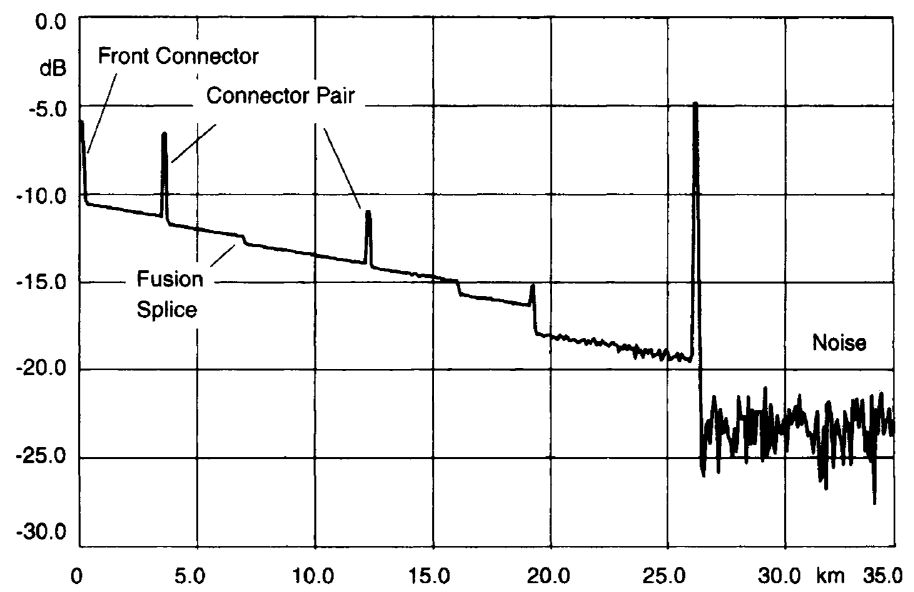
\includegraphics[width=0.9\textwidth]{otdr_sample.png}
	\caption{A sample OTDR measurement \cite{fer:oks}}
	\label{fig:otdr_sample}
\end{figure}
The loss introduced by Rayleigh scattering is manifested as a slope in the measured profile. Fibre attenuation can be easily retrieved by determining the slope. Other anomalies on the fibre can be observed, such as splicing and connector losses, Fresnel reflections off fibre ends, etc. All the losses at different points in the measurement fibre can be numerically measured on the oscilloscope screen.\\


\section{Optical frequency-domain reflectometry}

The \textit{optical frequency-domain reflectometry} (abbr. OFDR) is sometimes referred to as the \textit{frequency-modulated continuous-wave} (abbr. FMCW) method \cite{Farahani1999}\cite{Hartog2017}. The two types of OFDR are the coherent and incoherent OFDR. In coherent OFDR systems, the frequency (i.e. the wavelength) of the laser source is swept linearly. The laser is operated in a continuous-wave power regime. The reflected signal travels back to the source after time $2 \tau$, and is then mixed with the current laser signal by means of an electro-optic modulator. The resulting product will produce a signal at frequency
\begin{equation}
f_B = f(t - 2 \tau) - f(t) \textrm{.}
\end{equation}
For every $\tau$, the corresponding $f_B$ represents one point in space, identified as
\begin{equation}
z = v_g 2 f_B Y \textrm{,}
\end{equation}
where $Y$ is the frequency sweep rate. The mixing product is then acquired and subjected to fast-Fourier transform. The resulting signal is a profile, similar to that in the OTDR setup. In coherent OFDR, spatial resolution is determined by the sweep rate. However, if the sweep rate is kept sufficiently low, frequencies produced by mixing at the measurement side will be low, enabling acquisition by slower devices. \\

In incoherent OFDR, laser pulse amplitude is modulated by a sine signal. The frequency of that modulating signal is swept, instead of the wavelength of the laser itself. After the reflection, the signal arrives at the same type of electro-optic modulator. Mixing produces a signal whose frequency is a beating between the current modulation signal, and the modulation signal of the frame arriving back from the fibre under test. Same considerations for resolution and resulting acquisition frequencies apply as in the coherent setup. \\

The OFDR method enables very fine spatial resolution with sources that operate in a constant-wave regime, as opposed to impulse regime in OTDR. However, problems can occur as the strong signal, produced as a reflection against fibre end, overlaps the observed signal. SNR is thus degraded, notably for remote sections of the fibre under test. Peak power levels are limited by SRS threshold levels. However, in OTDR, the interaction of pump power with the scattered signal occurs along a small length of the fibre. In OFDR, the interaction is stronger, as all signals are continuously powered. Furthermore, in OFDR threshold will be dependent on the modulation frequency. The final effect is a notable amplitude modulation in Stokes signal. Also, the electronics operating at intermediate frequencies, measuring the reflected signal, are required to be highly-linear. This applies to laser electronics as well, in addition to the requirement on the laser to have a stable optical power level. To compensate for the deficiencies of electronics, a control channel can be introduced to serve as a continuous reference.

\section{Temperature sensing methods}

The described OTDR method can be applied for measuring other effects occurring in fibres. For distributed temperature sensing, one can either observe Brillouin or Raman scattering. As Brillouin scattering produces a relatively narrow-band frequency shift, it can be monitored by radio-frequency electronics. Raman scattering, on the other hand, produces a far larger frequency shift, whose components can be easily filtered by means of an optical filter. Information on temperature is obtained by monitoring the optical intensity of shifted signals. Therefore, a Raman scattering-based system utilizes simpler equipment and measurement method. \\

Chapter \ref{ch:fibres} identifies Stokes and anti-Stokes-shifted scattered signals produced by Raman effect. Powers of these signals are temperature-dependent, following Bose-Einstein distributions in equations \ref{eq:be-s} and \ref{eq:be-as}. The theoretical background enables measurement of only one of the scattered components, and calculating the absolute temperature from one of the signals. This requires precise knowledge of the parameters in \ref{eq:raman_beer} to ensure precise results. The resulting system would be material-dependent and difficult to calibrate. It can be noted that the two terms are largely equal, except for Bose-Einstein distribution terms, and terms involving scattering wavelengths. The \textit{Differential anti-Stokes Raman thermometry} method (abbr. DART) relies on measuring both Stokes and anti-Stokes scattering components, and finding the ratio of their powers numerically. Measured at point $z_0$, the ratio can be expressed as
\begin{equation}
R(T) = \frac{P_{AS}(z_0)}{P_S(z_0)} = \frac{G_\textrm{AS}}{G_\textrm{S}} \left( \frac{\lambda_S}{\lambda_{AS}} \right)^4 \exp\left( - \frac{\varDelta E}{k T} + \varDelta \alpha_P \, z_0 \right) \textrm{.}
\end{equation}
Terms $G_\textrm{S}$ and $G_\textrm{AS}$ are gain coefficients of measurement chains on Stokes and anti-Stokes channels, respectively. These include different photodiode responsivities, gains and probe attenuations. Term $\varDelta \alpha_P$ is the difference of attenuation coefficients at pump wavelength and scattered wavelengths. The characteristic of the $\alpha(\omega)$ function is assumed to be linear, and Raman spectrum generally symmetrical. Therefore, only one calculation for $\varDelta \alpha$ should be performed. Finally, temperature in kelvins at position $z_0$ is found as
\begin{equation} \label{eq:stokes_temperature}
T(z_0) = \frac{\varDelta E}{k \, \ln \left[ \frac{I_S}{I_{AS}} \frac{\Re_{AS}}{\Re_S} \frac{G_{AS}}{G_S} \left(\frac{\lambda_S}{\lambda_{AS}}\right)^4 \right] + \varDelta \alpha_P z_0 } \textrm{,}
\end{equation}
where $\Re_S$ and $\Re_{AS}$ are responsivities of photodiodes at effective Stokes and anti-Stokes wavelengths, respectively.


% --------------------------------------

\setcounter{stranica}{\thepage}
\addtocounter{stranica}{1}

\end{document}